%----------------------------------------------------------------------------
\chapter{Elméleti alapok}\label{sect:elmeleti_alapok}
%----------------------------------------------------------------------------

\texttt{+++ bevezeto a fejezethez +++}

\texttt{+++ Hough-t megvagni? +++}

\bigskip

\texttt{+++ melyik szakaszban mi van +++}

%,,,,,,,,,,,,,,,,,,,,,,,,,,,,,,,,,,,,,,,,,,,,,,,,,,,,,,,,,,,,,,,,,,,,,,,,,,,,
\section{Hough-transzformáció}\label{sect:hough}
%,,,,,,,,,,,,,,,,,,,,,,,,,,,,,,,,,,,,,,,,,,,,,,,,,,,,,,,,,,,,,,,,,,,,,,,,,,,,

Képfeldolgozási szûrõk, függvények segítségével viszonylag könnyen előállíthatjuk a képtérben számunkra érdekes pontok halmazát. Azokat a pontokat, amelyek valamilyen magasabb absztrakciós szintû képjellemzõhöz kapcsolódnak: például a tárgyak, alakzatok formáját megadó kontúrok pontjait. Ha viszont szeretnénk ,,megérteni'' is a képet, az ilyen formák automatikus és robusztus felismerése szinte elengedhetetlen.

A valóságban a kontúrok pontjai azonban csak többé-kevésbé illeszkednek ideális formákra (egyenesekre, körökre, vagy egyéb görbékre): az éleket torzíthatja zaj, egyes élpontok hiányozhatnak, vagy a felismerni kívánt formák kismértékben el is térhetnek az ideálistól. A kép analízise szempontjából azonban ezzel együtt is nagyon értékes információt rejthetnek magukban, ezt az információt pedig hasznos lenne kinyerni. Viszont egyáltalán nem triviális probléma a valamilyen szempontból összetartozó (például egy egyenesre, vagy egy körvonalra esõ) pontok csoportosítása.

\begin{figure}[!ht]
\centering
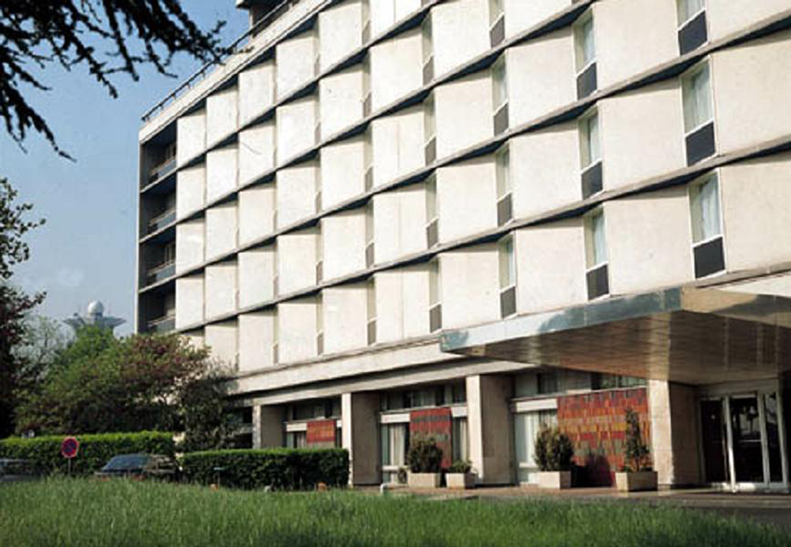
\includegraphics[width=67mm, keepaspectratio]{figures/houghline_building_1.png}\hspace{1cm}
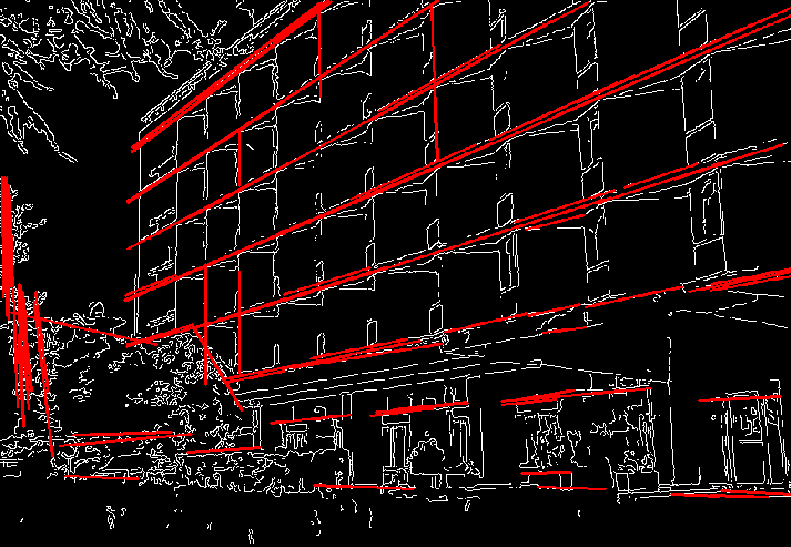
\includegraphics[width=67mm, keepaspectratio]{figures/houghline_building_2.png}
\caption{Egyenesek keresése Hough-transzformáció használatával.\\Forrás: \url{http://href.hu/x/c91h}}
\label{fig:houghlines}
\end{figure}

A Hough-transzformáció erre a problémára kínál megoldást. Feladata egyszerû formák, úgymint egyenesek, körök, ellipszisek keresése képeken. Az alakzatok keresését a transzformáció egy ún. paramétertérben végzi egy szavazási mechanizmus segítségével. A felismert potenciális objektumok az akkumulátortér -- a paramétertér egyfajta futás közbeni leképezése -- lokális maximumai alapján adódnak.

\bigskip

Történelmi áttekintésként megjegyezhetjük, hogy a Hough-transzformációt Paul~Hough alkotta meg 1959-ben buborékkamra-fényképek gépi analíziséhez \cite{hough_eredeti}. Ebben a cikkben Hough még csak egyenesek felismerésérõl beszél. A manapság használt transzformációt Richard~Duda és Peter~Hart fejlesztette ki 1972-ben ,,általánosított Hough-transzformáció'' néven \cite{hough_duda}, tíz évvel azután, hogy Paul Hough szabadalmaztatta módszerét. Az õ kiegészítésük már lehetõvé tette, hogy a transzformáció nemcsak egyenesek, hanem körök és más analitikusan leírható görbék keresésére is felhasználható legyen.

A gépi látás felhasználói körében azonban igazán csak Dana~H.~Ballard 1981-es cikke \cite{hough_ballard} nyomán lett népszerû, aki a transzformáció még további felhasználási lehetõségeit vetette fel. Eredményeinek köszönhetõen a módszer analitikusan nem (vagy csak nehezen) leírható formák keresésére is alkalmazhatóvá vált. Félreértésekre adhat okot, hogy mind Duda és Hart, mind Ballard az ,,általánosított'' megnevezést használja a módszer általuk kitalált kiegészítéseinek. A továbbiakban az ,,általános'' jelzõt a Duda--Hart-féle kiegészítés megnevezésére használom, ahol Ballard módszerérõl esik szó, azt külön jelzem.

\bigskip

A transzformáció általános formájában tehát analitikusan leírható formák keresésére használható. A legegyszerûbb ilyen forma az egyenes, ennek segítségével érthetõ meg legkönnyebben az algoritmus mûködési elve. A \sectref{egyenesek_keresese} szakaszban ezért az egyenesek keresésének elméletét foglalom össze. Ezen elv késõbb már könnyen kiterjeszthetõ tetszõleges formák keresésére, különös tekintettel a pupilla-keresés szempontjából fontos körkeresési problémára, amelyre a \sectref{korkereses} szakaszban térek ki. A \sectref{kiegeszitesek} szakaszban szót ejtek még a módszer további kiegészítési lehetõségeirõl, majd a \sectref{hough_osszefoglalas} szakaszban összefoglalom a Hough-transzformáció használatának korlátait, elõnyeit és hátrányait.


%............................................................................
\subsection{Egyenesek keresése}\label{sect:egyenesek_keresese}
%............................................................................

%. . . . . . . . . . . . . . . . . . . . . . . . . . . . . . . . . . . . . .
\subsubsection{Egyenes-reprezentációk}\label{sect:egyenes_reprezentaciok}
%. . . . . . . . . . . . . . . . . . . . . . . . . . . . . . . . . . . . . .

Egyenesek leírására többféle modell használható. Az egyenes ,,klasszikus'' modellje Descartes-koordinátarendszerben az

\begin{align}\label{eq:egyenes_klasszikus}
y = m \cdot x + b
\end{align}

reprezentáció, ahol $ m $ az egyenes meredeksége (iránytangense), a $ b $ konstans az ordinátatengely-metszet, vagyis az egyenes és az $ y $ tengely metszéspontja.

A \eqref{egyenes_klasszikus} egyenlettel megadott modellel az a probléma, hogy a koordinátarendszer $ y $ tengelyével párhuzamos, vagy ahhoz közelítõ egyenesek leírására nem használható $ m $ végtelen nagy értéke miatt. Nem szerencsés azonban az ilyen ,,függõleges'' egyenesek kizárása a számításból. Ennek kiküszöbölésére -- jelen esetben -- jobb modellként segítségül hívhatjuk a \textbf{Hesse-féle normálalakos} reprezentációt. Ez az

\begin{align}\label{eq:egyenes_hesse}
r = x \cdot \cos \theta + y \cdot \sin \theta
\end{align}

egyenlettel adja meg a kívánt egyenest, ahol $ r $ az origótól mért távolságot, $ \theta $ pedig az egyenes pozitív valós féltengellyel bezárt szögét jelenti (lásd \figref{repr_line} ábra). Ezzel a megvalósítással már nem ütközik akadályba az $ y $ tengelyhez közelítõ egyenesek modellezése.

\begin{figure}[!ht]
\centering
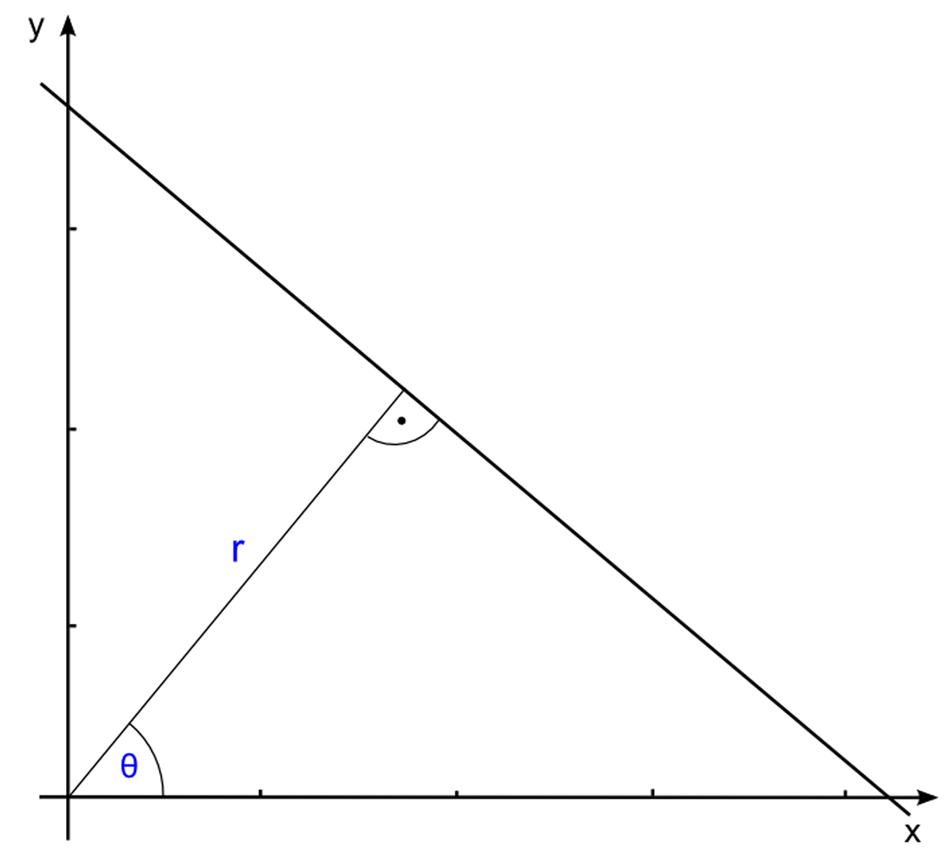
\includegraphics[width=80mm, keepaspectratio]{figures/repr_line.png}
\caption{Egyenes jellemzése $ r $ és $ \theta $ paraméterekkel.}
\label{fig:repr_line}
\end{figure}

\bigskip

Érdekességként megemlíthetõ, hogy bár nyilvánvalónak látszik a Hesse-féle normálalak elõnyösebb volta, Paul Hough eredeti szabadalmában\footnote{U.S. Patent 3,069,654 -- \url{http://www.google.com/patents?q=3069654}} mégis az $ y = m \cdot x + b $ formát használta az egyenesek jellemzésére. Az $ (r, \theta) $ paraméterezés Duda és Hart már hivatkozott cikke nyomán vált általánosan használttá. \cite{hough_duda}

%. . . . . . . . . . . . . . . . . . . . . . . . . . . . . . . . . . . . . .
\subsubsection{A paramétertér és az akkumulátor}\label{sect:parameterter_akkumulator}
%. . . . . . . . . . . . . . . . . . . . . . . . . . . . . . . . . . . . . .

Minden képtérbeli egyenes tehát \eqref{egyenes_hesse} felhasználásával megfeleltethetõ a paramétertérben egy $ (r, \theta) $ párral jellemzett pontnak. Az egyértelmû megfeleltetés végett két lehetõségünk is adódik a paraméterek korlátainak megválasztására. Ezek formálisan

\begin{align}\label{eq:param180}
\theta \in \left[ 0,180^{\circ} \right) \quad \wedge \quad r \in \mathbf{R}
\end{align}

vagy

\begin{align}\label{eq:param360}
\theta \in \left[ 0,360^{\circ} \right) \quad \wedge \quad r \geq 0
\end{align}

Az $ (r, \theta) $ párok terét \textbf{paramétertérnek}, vagy \textbf{Hough-térnek} hívjuk. A paramétertér dimenzióját az ismeretlen paraméterek száma adja, egyenesek esetében ez tehát kettõ.

Egy $ (x,y) $ ponton keresztül végtelen sok egyenes húzható, és minden egyenes kielégíti a \eqref{egyenes_hesse} összefüggést. Ezek az egyenesek a paramétertérben ábrázolva egy szinusz-jellegû görbét alkotnak. Természetesen nem határozhatunk meg tetszõleges pontossággal egy pontot, és nem is vehetünk számításba minden (végtelen számú) olyan egyenest, ami az adott ponton átmegy. Szükség van ezért a paramétertér diszkretizálására.

\bigskip

A paramétertér gyakorlati (kvantált) reprezentációja az \textbf{akkumulátor}. Az akkumulátor egy tömb, dimenziószáma megegyezik a paramétertér dimenziószámával.

A tömbök indexelése egész számokkal történik ezért az $ r $ paramétert egész számokra célszerû kvantálnunk. A $ \theta $ paraméter kvantálásához pedig a végtelen sok egyenes figyelembe vétele helyett az $ (x,y) $ koordinátán keresztül húzhatunk egyeneseket $ \varDelta \theta $ fokonként. Ebbõl következõen a \eqref{param180} vagy \eqref{param360} összefüggések alapján az akkumulátor ezen dimenzióját $ 180^{\circ} / \varDelta \theta $, illetve $ 360^{\circ} / \varDelta \theta $ darab diszkrét részre osztja. A $ \varDelta \theta $ paraméter megválasztásával, a módszer ,,finomságát'' növelhetjük. Például $ \varDelta \theta = 5^{\circ} $ választás esetén a transzformáció csak a pozitív valós féltengellyel $ 0, 5, 10, ... $ fokot bezáró egyenesek felismerésére képes. Túl kis érték választása esetén viszont az eljárás memória- és idõigénye fog az egekbe szökni. A $ \varDelta \theta $ érték gondos megválasztásával tehát a pontosság és gyorsaság egy lehetõleg optimális értékét kell meghatároznunk.

Gyakorlati szabályként elmondható, hogy 1 fok pontosságnál többre ritkán van szükség. Túl vastag vonalak (amik pedig logikailag összefüggõ egyenesek), zajos kép, vagy túl rövid vonalszakaszok esetén így is romlik a felismerés esélye. Hogy miért, arra a következõ szakasz -- a szavazási mechanizmus ismertetése -- ad választ.

%. . . . . . . . . . . . . . . . . . . . . . . . . . . . . . . . . . . . . .
\subsubsection{A keresés folyamata}\label{sect:kereses_folyamata}
%. . . . . . . . . . . . . . . . . . . . . . . . . . . . . . . . . . . . . .

A továbbiakban tételezzük fel, hogy a kép bináris, és megfelelõen elõfeldolgozott (pl. élkeresés, küszöbözés), azon már csak a felismerni kívánt egyenesek pontjai találhatóak. A háttér képpontjait jelölje a 0 érték, az érdekes pontokat tartalmazó elõtér képpontjai legyenek 1 értékûek.

A keresés folyamán bejárjuk a képteret pixelrõl pixelre. A 0 értékû képpontok biztosan nem részei egy képen található egyenesnek sem, ezért ezekkel nem kell foglalkozunk. Ha 1 értékû pixelt találunk az $ (x,y) $ helyen, az potenciálisan része lehet egy, a képen található egyenesnek. Az akkumulátor minden $ \theta $ értékhez (pl. fokonként) meghatározzuk az $ (x,y) $ ponton átmenõ, $ \theta $ irányú egyenes origótól vett $ r $ távolságát a \eqref{egyenes_hesse} összefüggés alapján. Az akkumulátortömb értékét minden így kiszámolt $ (r,\theta) $ indexekkel jelölt helyen megnöveljük ($ r $ meghatározásánál természetesen a tömb kvantáltságát figyelembe véve). Ezt a folyamatot úgy is mondhatjuk, hogy az $ (x,y) $ pont a kiszámított $ (r, \theta) $ pontok halmazára, vagyis ezen paraméterek által a képtérben képviselt egyenesekre \textbf{,,szavaz''}.

Az algoritmus elsõ fázisának lefutása után az akkumulátortömböt kell vizsgálnunk. Optimális esetben a képen egy egyenesre esõ pixelek mindegyike (a többi más szavazatuk mellett) szavazott a ,,valódi'' egyenest jelentõ $ (r, \theta) $ párra. Az akkumulátortömb maximális értékû $ (r, \theta) $ elemei adják meg tehát a képen található egyeneseket. A zaj, az esetleg több pixel széles vonalak, és a kvantálási pontatlanság miatt azonban célravezetõbb \textbf{lokális maximumokat} (lásd \figref{houghparam} ábra) keresni az akkumulátortömbben így meghatározva a \textbf{legvalószínûbb} egyenesek $ r $ és $ \theta $ paramétereit.

\begin{figure}[!ht]
\centering
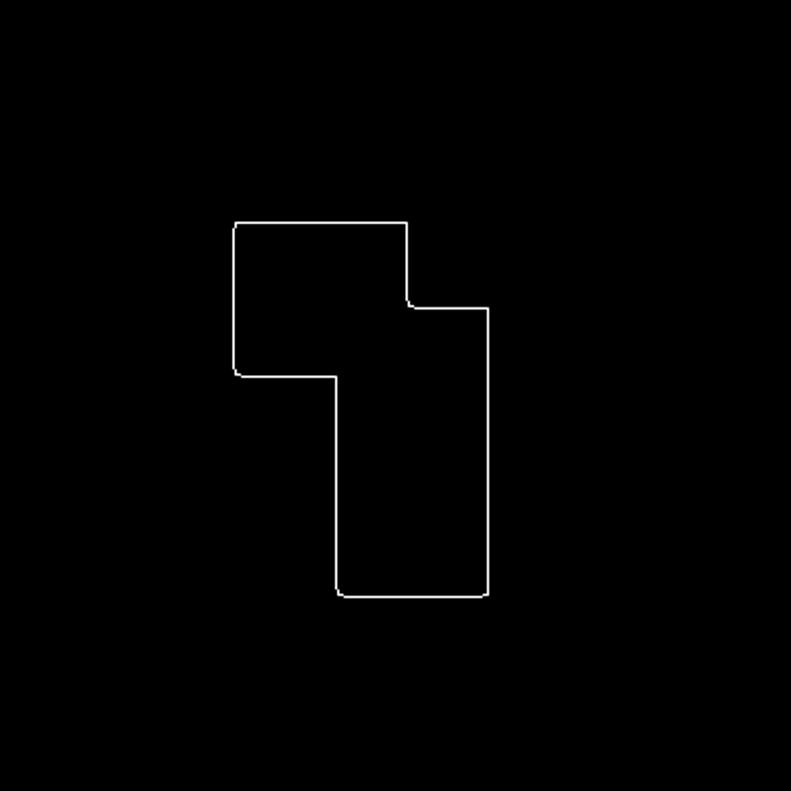
\includegraphics[width=67mm, keepaspectratio]{figures/houghparam_1.png}\hspace{1cm}
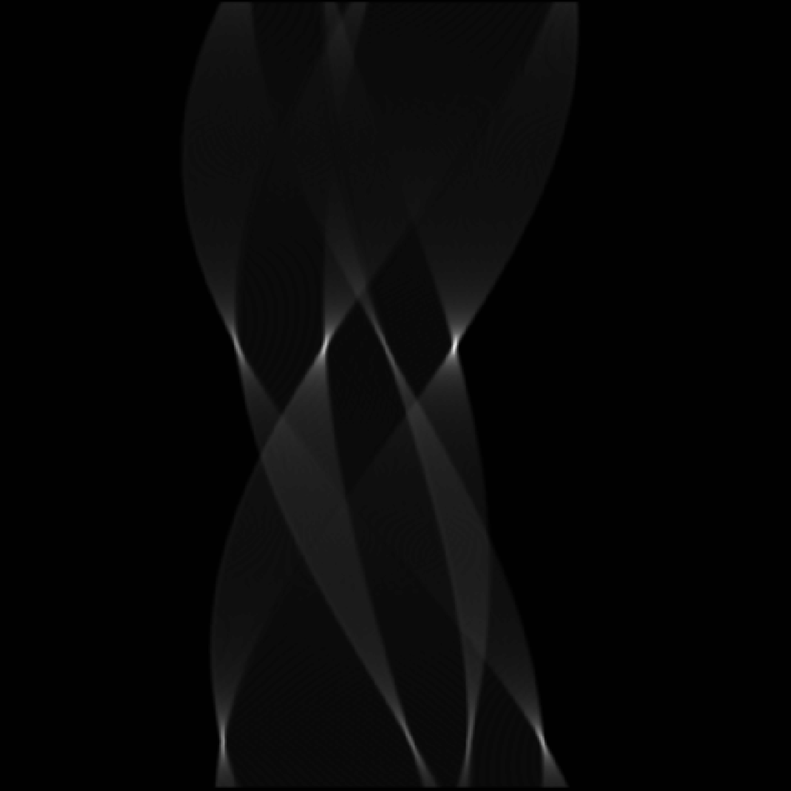
\includegraphics[width=67mm, keepaspectratio]{figures/houghparam_2.png}
\caption{A képtér (balra) és az ebbõl származó paramétertér (jobbra) egyenesek keresése során.\\Forrás: \url{http://href.hu/x/c91i}}
\label{fig:houghparam}
\end{figure}

Az elõzõ szakasz végén felvetett problémát most már megválaszolhatjuk. A túl nagy zaj miatt megnõ azon képpontok száma, amik nem részei egy egyenesnek sem. Azonban szavazni ezek a képpontok is szavaznak, ezzel mintegy ,,háttérzajt'' adva az akkumulátortömbnek. Túl vastag vonalak esetén pedig több, látszólag helyes paraméterezésû egyenes adódna ugyanarra a vonalra (pl. egymással a vonalon belül párhuzamos egyenesek, de kellõen vastag vonal esetén akár ,,átlós'' egyenesek is). Az elsõ esetben az akkumulátortömb elemeinek átlagos értéke nõ meg, a második esetben pedig a sok egymáshoz közeli szavazat miatt lokális maximumok értékei kerülnek közelebb az átlagos tömbértékekhez. Mindkét esetben nehezebbé válik a lokális maximumok pontos meghatározása, ez pedig drasztikusan csökkentheti a keresés pontosságát.

%............................................................................
\subsection{Körkeresés}\label{sect:korkereses}
%............................................................................

%. . . . . . . . . . . . . . . . . . . . . . . . . . . . . . . . . . . . . .
\subsubsection{Körök reprezentációja}\label{sect:korok_reprezentacioja}
%. . . . . . . . . . . . . . . . . . . . . . . . . . . . . . . . . . . . . .

A körökhöz megfelelõ reprezentáció megtalálásához még annyit sem kell törnünk a fejünket, mint az egyeneseknél tettük. Descartes-koordinátarendszerben az $ (x_{0}, y_{0}) $ középpontú $ r $ sugarú körvonal pontjait az

\begin{align}\label{eq:kor_koogeom}
( x - x_{0})^{2} + (y - y_{0})^2 = r^2
\end{align}

egyenlet adja meg (\figref{repr_circle} ábra). Szögfüggvények használatával az \eqref{kor_koogeom} egyenletet átalakíthatjuk

\begin{align}\label{eq:kor_param}
x &= x_{0} + r \cdot \cos \theta \nonumber \\
y &= y_{0} + r \cdot \sin \theta
\end{align}

formára, ahol $ (x_{0}, y_{0}) $ szintén a kör középpontjának koordinátái, $ r $ a sugár, $ \theta $ pedig a körvonal egy pontját a kör középpontjával összekötõ szakasz pozitív valós féltengellyel bezárt szögét jelenti.

\begin{figure}[!ht]
\centering
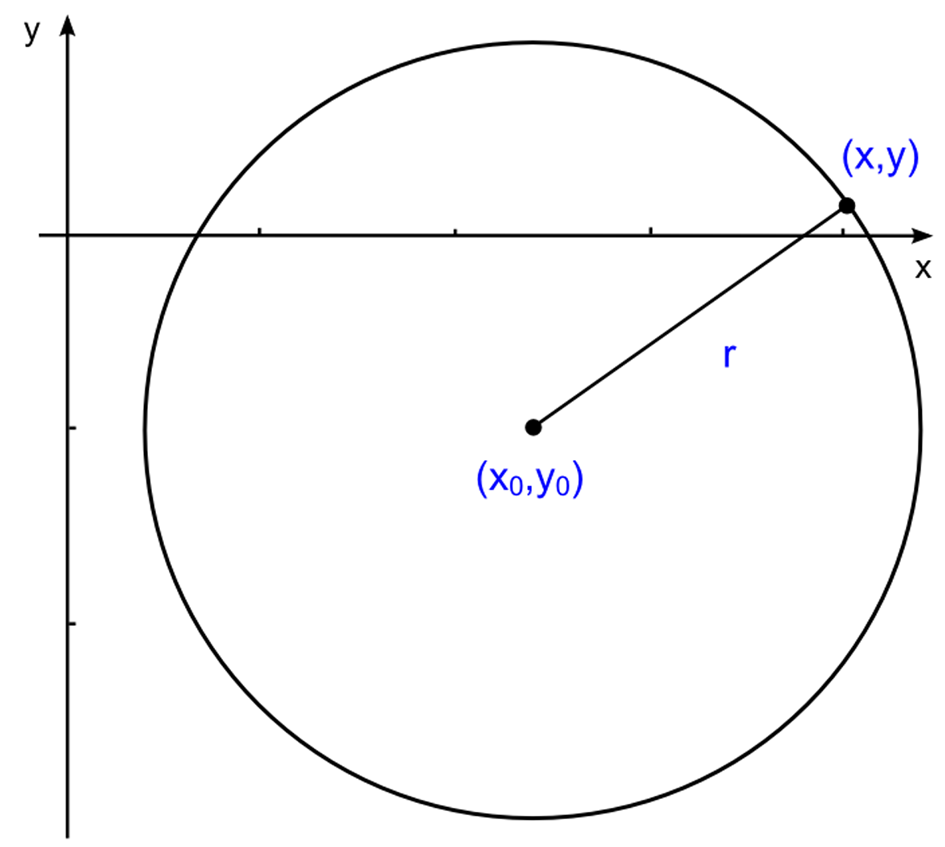
\includegraphics[width=80mm, keepaspectratio]{figures/repr_circle.png}
\caption{Körök reprezentációja.}
\label{fig:repr_circle}
\end{figure}

%. . . . . . . . . . . . . . . . . . . . . . . . . . . . . . . . . . . . . .
\subsubsection{A paramétertér körök esetében}\label{sect:korok_parameterter}
%. . . . . . . . . . . . . . . . . . . . . . . . . . . . . . . . . . . . . .

Látható, hogy körök esetében már csak akkor elegendõ két paraméter -- az $ (x_{0}, y_{0}) $ középpont-koordináták -- a forma leírásához, ha elõre adott sugarú köröket keresünk, vagyis $ r $ konstans. Ez azonban csak bizonyos esetekben használható, általános esetben túl nagy megkötést jelent. Tehát a paramétertér dimenziószámát növelnünk kell: az $ r $ sugárparaméter dimenziójával együtt az már \textbf{három dimenziós lesz}.

A paraméterteret az akkumulátor tömb mivoltából adódóan itt is egész számokra kell kvantálnunk. Körkeresés esetén az akkumulátor tehát egy három dimenziós tömb, amely a középpont két koordinátájának és a sugárnak egész értékeivel indexelhetõ. Már a pontos algoritmus ismerete nélkül is látszik, hogy a potenciális körök keresése jóval komplexebb mûvelet az ismeretlen paraméterek magasabb száma miatt.

%. . . . . . . . . . . . . . . . . . . . . . . . . . . . . . . . . . . . . .
\subsubsection{A körkeresés folyamata}\label{sect:korok_keresese}
%. . . . . . . . . . . . . . . . . . . . . . . . . . . . . . . . . . . . . .

Az alaphelyzet legyen az egyenesek keresésekor felállított: a felismerni kívánt körvonalak képpontjai legyenek 1, a háttér felismerés szempontjából érdektelen képpontjai pedig legyenek 0 értékûek.

A bejárás során 1 értékû pixelt találva jóval több számítani valónk van, mint egyenesek esetében. Az akkumulátor \textbf{összes lehetséges $ r $ sugárparaméterére} meg kell határoznunk a potenciális körök középpontjait. Ehhez felhasználjuk az \eqref{kor_param} összefüggéseket $ r $ és $ \theta $ ismeretében ($ \theta $ lehetséges értékeinek megválasztása -- tipikusan például fokonként -- azonos elven történhet a \sectref{parameterter_akkumulator} szakaszban olvashatóakkal).

Hogy próbálhatjuk meg csökkenteni a rengeteg számítást? Egyfelõl \textbf{korlátozhatjuk} $ r $ lehetséges értékeinek halmazát. Az értékeknek $ r_{min} $ alsó és $ r_{max} $ felsõ korlátot adva a keresést a két érték közötti sugarú körökre szûkíthetjük. Némi elõzetes információ birtokában (körülbelül, vagy a kép oldalainak arányában mekkora köröket kell keresnünk) jelentõsen csökkenthetõ a számítási idõ- és tárigény.

Másfelõl pedig felhasználhatunk lokális információkat is: a vizsgálat alatt lévõ képpont egy adott ablaknyi környezetét vizsgálva, meghatározhatjuk a körvonal adott pontbeli \textbf{gradiensét}. Ez az információ felhasználható a középpont keresésében, ugyanis a kör középpontjának a körvonalpont normálisán kell feküdnie. Így, ha nem is egyetlen kitüntetett irányra, de a számítási pontatlanságot és a zajt figyelembe véve egy szûk tartományra korlátozhatjuk a keresett körközéppontok irányát. Ez a választott tartomány méretével fordított arányosságban csökkenti a szükséges számítások számát. Példának okáért, ha a kiszámított gradiens segítségével akár csak 90 fok pontossággal meg tudjuk határozni a pontban vett normális irányát, a számítások háromnegyedét nem kell elvégeznünk, ráadásul az akkumulátortömb sem telítõdik feleslegesen olyan paraméterekkel, amelyekbõl biztosan (vagy elég nagy valószínûséggel) nem fog helyes megoldás születni.

%. . . . . . . . . . . . . . . . . . . . . . . . . . . . . . . . . . . . . .
\subsubsection{Variációk körkeresésre}\label{sect:korok_kiegeszites}
%. . . . . . . . . . . . . . . . . . . . . . . . . . . . . . . . . . . . . .

A körkeresésre használt Hough-transzformáció további kiegészítéseivel találkozhatunk H. K. Yuen \textit{et al} hivatkozott cikkében \cite{hough_circles}. A cikkben az elõzõ alfejezetben ismertetett sztenderd változat mellett még további négy módosulat vizsgálatát és ezek összehasonlítását végzik el a szerzõk. Ezek közül a cikkben ,,2-1 Hough-transzformációnak'' néven hivatkozott módszert emelném ki, a késõbbiek során ugyanis ennek fontos szerepe lesz. Elnevezésként a cikkben használt ,,21HT'' rövidítést fogom használni.

A \textbf{21HT} módszer a \cite{hough_21_davies} és \cite{hough_21_illingworth} számon hivatkozott cikkekben volt elõször használatos. A kiegészítés felhasználja a rendelkezésre álló gradiens-információt (lásd: \sectref{korok_keresese}), és ennek ismeretében pedig a problémát két részre osztja. Mivel a kör középpontjának a körvonalpontok normálisán kell feküdnie, ezen normálisok közös metszéspontja valójában tehát meghatározza a középpontot. Egy kétdimenziós akkumulátortömb pedig elég minden pont saját normálisára esõ szavazatainak nyilvántartásához. Ezután a sugár meghatározása a következõ módszerrel történhet: meghatározzuk minden pont és az elõzõ lépésben kiszámított középpont-jelölt távolságát, majd ezekbõl az információkból egy sugár-hisztogramot állítunk elõ. Ennek vizsgálatával már meghatározhatjuk a középpontokhoz tartozó sugarakat is. A módszer tárigénye az eredeti megközelítéshez képest jóval kisebb, hiszen csak egy \textbf{2D akkumulátort} és egy \textbf{1D hisztogramot} kell használnunk -- innen a módszer ,,2-1'' elnevezése.

Eredmények tekintetében az összehasonlító cikk szerint a 21HT módszer felveszi a versenyt a sztenderd megoldással. Igaz, hogy a kétfázisú számítás miatt az elsõ fázisban összeszedett hiba szükségszerûen rárakódik a második fázisra, ezt a pontatlanságot ellensúlyozni tudja a módszer jelentõsen kisebb tárigénye.

%............................................................................
\subsection{Kiegészítések}\label{sect:kiegeszitesek}
%............................................................................

A meglévõ módszer továbbfejlesztésekor két irányba is elindulhatunk:

\begin{enumerate}
 \item egyrészt növelhetjük az algoritmus teljesítõképességét,
 \item másrészt bõvíthetjük a felismerhetõ formák halmazát.
\end{enumerate}

Ebben a szakaszban mindkét lehetséges fejlesztési irány eredményeirõl szeretnék röviden beszámolni a témában fellelhetõ szakirodalom felhasználásával.

\bigskip

Az elsõ irányba mutató fejlesztések közül néhánnyal már találkozhattunk jelen dolgozat keretein belül is. Az \sectref{korok_keresese} alszakaszban elõkerült a gradiensinformáció felhasználása és az elõzetes tudás alapján történõ megfelelõ korlátok bevezetése a számítás gyorsítása végett. Ebben a témában mindenképp megemlítendõ még a kernel alapú Hough-transzformáció.

A \textbf{kernel alapú megvalósítás} lehetõségét a szerzõk -- Fernandes és Oliveira -- 2008-as cikkükben \cite{hough_fernandes} vetették fel, tehát a módszer meglehetõsen friss. Állításuk szerint valósidejû mûködés érhetõ el viszonylag nagy képek esetén is a szavazási protokoll továbbfejlesztésének köszönhetõen. A módszer egyeneskereséskor az $ (r, \theta) $ paraméterezésen nem változtat, de nem önmagukban álló pontokat, hanem körülbelül egy irányban álló pixelek klasztereit (csoportjait) veszi figyelembe. Minden klaszterben egy megfelelõ irányba forgatott elliptikus Gauss-kernellel végzett konvolúció hivatott a csoportra vonatkozó bizonytalanságot modellezni. Ez a megközelítés nemcsak hogy a szavazatok számának csökkentésével képes az algoritmus sebességét növelni, hanem a protokollnak köszönhetõen sokkal tisztább akkumulátort is eredményez. A háttérzajtól mentes tömbben pedig jóval könnyebben tudjuk a lokális maximumokat detektálni. Ezzel összességében az eddigieknél gyorsabb és pontosabb egyenesdetektálást tudunk kivitelezni.

\bigskip

Felismerhetõ formák tekintetében a módszer bõvíthetõ az általános analitikus 2D görbék mellett 3D képeken testek felismerésére. Ezen kívül semmiképp nem hagyhatjuk szó nélkül a Ballard-féle általánosított Hough-transzformációt sem.

Három dimenzióban a \textbf{testek felismerése} a két dimenziós esetekhez hasonlóan történik -- hasonló buktatókkal és legtöbbször további járulékos memória- és számításigénnyel. Síkoknál például az egyenesekhez hasonlóan a megszokott reprezentáció nem használható függõleges síkok keresésére. A megoldást ebben az esetben a gömbi koordinátarendszerre való átállás jelenti, ahol a sík már normálvektorával és az origótól való távolságával jellemezhetõ (a paramétertér tehát három dimenziósra adódik). Gömbök, hengerek, ellipszoidok keresése szintén a két dimenziós esetek tapasztalatainak felhasználásával történhet. Az új, akár térbeli formák keresése kombinálható az eddig megismert teljesítménynövelõ eljárásokkal: a már megismer eljárások használhatók a keresés során, természetesen adott esetben három dimenzióra vonatkoztatva azokat.

Dana H. Ballard általánosított transzformációja \cite{hough_ballard} -- amint az már jelen dolgozat keretein belül is elõkerült -- lehetõvé teszi modelljükkel reprezentált általános objektumok felismerését a \textbf{mintafelismerés} alapelvét kihasználva. A modell elõfordulásainak keresése a képtérben -- ahogy Ballard megmutatta -- szintén megoldható paraméterek akkumulálásával. Válasszuk ezen paramétereknek a modellt a képtérbe átvivõ transzformáció (vagy transzformációk) paramétereit! Például ha csak a modell pozícióját keressük, akkor mindössze eltolási paramétereket kell figyelembe vennünk, ezek akkumulálásával a megszokott módon és eredményességgel ismerhetjük fel az adott objektum helyzetét. Azonban a módszer a transzláció (eltolás) invariancia mellett rotáció (forgatás) és skálázás (méret) invariánssá is tehetõ, igaz a paramétertér dimenziószámának növelése árán. Láthatjuk, hogy a mintafelismerés és a szavazási mechanizmus elõnyeinek ötvözésével ez az eljárás igazán komoly fegyver lehet a képfeldolgozási eszköztárunkban.

\begin{figure}[!ht]
\centering
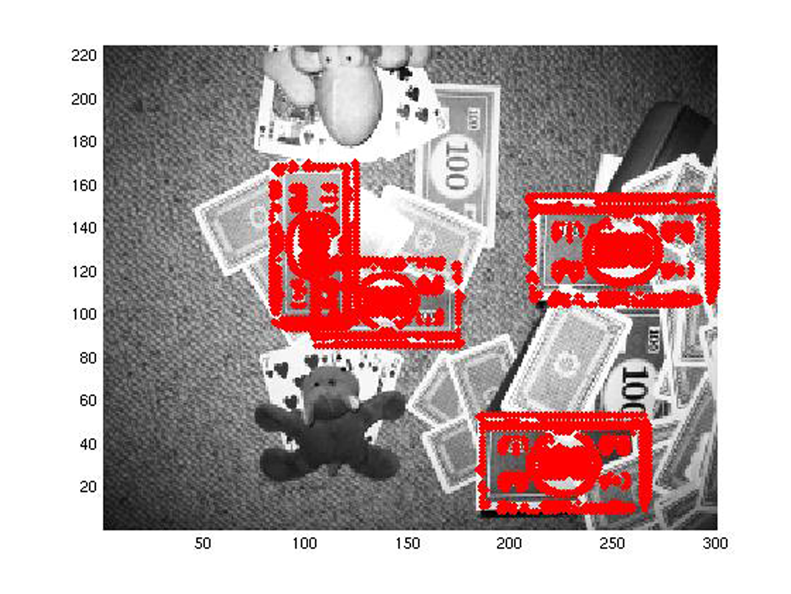
\includegraphics[width=67mm, keepaspectratio]{figures/generalhough_money_1.png}\hspace{1cm}
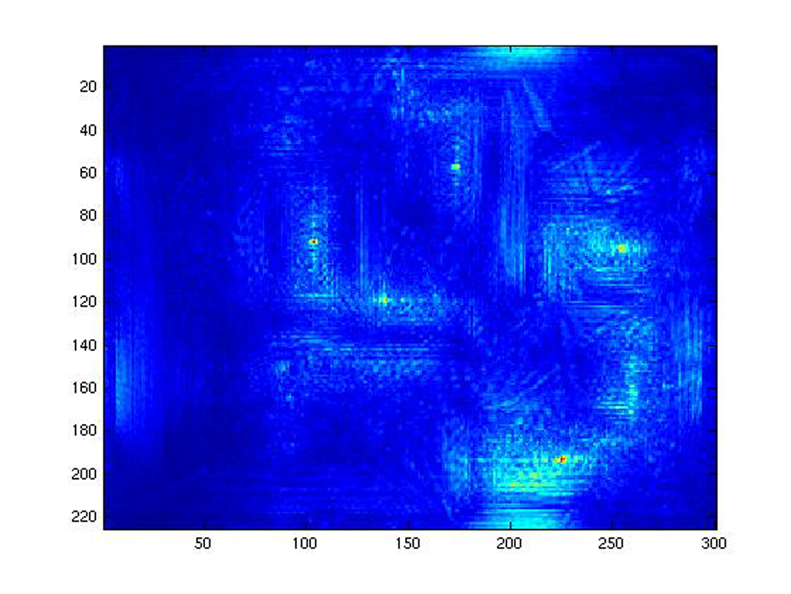
\includegraphics[width=67mm, keepaspectratio]{figures/generalhough_money_2.png}
\caption{Kép- és paramétertér az általánosított Hough-transzformáció használata közben.\\Forrás: \url{http://href.hu/x/c91m}}
\label{fig:generalhough}
\end{figure}

%............................................................................
\subsection{Összegzés}\label{sect:hough_osszefoglalas}
%............................................................................

Az eddigiek alapján látszik, hogy a transzformáció felhasználhatóságának szûk keresztmetszetét leginkább a nagy számításigénye adja. Ez egyben legfõbb \textbf{hátránya} is: a számításigény a paramétertér dimenziószámának, vagy a kép méretének növekedésével egyre csak növekszik. A dimenziók száma tehát korlátot ad a transzformáció gyakorlati felhasználhatóságának, ezért eredeti formájában leginkább csak egyenesek, vagy körök keresésére használják. A körök keresésének lehetõsége azonban kielégítheti a pupillakövetési probléma által támasztott követelményeket. A követés során \textbf{elõnyére} válhat, hogy a szavazási mechanizmus használata miatt meglehetõsen zajos képeken is képes lehet a pupillakontúr megbízható felismerésére. Nem mesterségesen elõállított tesztesetekben -- hiszen pupillakövetés esetén csak ennek van értelme -- pedig ez korántsem elhanyagolható szempont.


\newpage
%,,,,,,,,,,,,,,,,,,,,,,,,,,,,,,,,,,,,,,,,,,,,,,,,,,,,,,,,,,,,,,,,,,,,,,,,,,,,
\section{Objektumdetektálás és -követés}\label{sect:objdetect}
%,,,,,,,,,,,,,,,,,,,,,,,,,,,,,,,,,,,,,,,,,,,,,,,,,,,,,,,,,,,,,,,,,,,,,,,,,,,,

\texttt{+++ kis bevezeto +++}

%............................................................................
\subsection{A Viola--Jones objektumdetektor}\label{sect:viola}
%............................................................................

A Paul Viola és Michael Jones által 2001-ben elővezetett \cite{vj} Viola--Jones objektumdetektor az első olyan objektumfelismerő rendszer, megközelítheti, vagy akár teljesítheti is a valósidejű feldolgozás által támasztott követelményeket. A rendszer eleinte arcdetektálás céljából készült, de mint kiderült, működése könnyen általánosítható, így megfelelő tanítás után bármilyen objektum felismerésére képes lehet.

\begin{figure}[!ht]
\centering
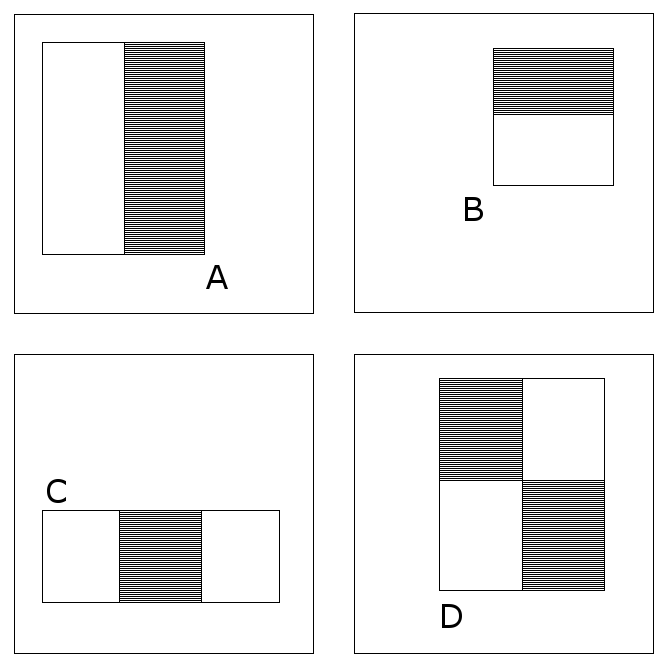
\includegraphics[width=50mm, keepaspectratio]{figures/features.png}
\caption{A Viola és Jones által használt jellemzőtípusok.\\Forrás: \cite{vj}}
\label{fig:features}
\end{figure}

Az osztályozó úgynevezett \emph{jellemzőkkel} (features) dolgozik, amelyek téglalap alakú területeket alapul véve a bennük lévő képpontok összegét jelentik. Ebben a formában a jellemzők rokonságot mutatnak a Haar bázisfüggvényekkel, amelyek az objektumdetektálásban korábban meghatározó \emph{wavelet transzformációnál} használatosak. Lehetséges jellemzőtípusokat mutat be a \figref{features} ábra.

A jellemző-alapú, úgynevezett \emph{integrális} képreprezentáció esetén az egyes jellemzők ugyan nagyon egyszerűek, viszont konstans időben kiértékelhetők. A jellemzők gyors értékelhetősége azonban nem kompenzálja nagy számukat. Minden egyes területre minden jellemzőt kiértékelve csökkenne a rendszer használatával nyert előny. Ennek kiküszöbölésére a betanítási fázisban a Viola--Jones detektor az AdaBoost \cite{freund} eljárás egy módosított változatát alkalmazza, amely segít kiválasztani a leginkább fontos jellemzőket, valamint korlátokat ad a kész osztályozó általánosító képességére.

Ha csak az AdaBoost eljárás által kiválasztott fontos jellemzőket értékeljük ki, a rendszer alapesetben akkor sem képes a valós idejű osztályozásra. Ennek kivédésére a tanítási folyamatban az egyes elemi osztályozókat egymás után kötik (kaszkádosítják), és minden osztályozó bemenetére csak azok a minták jutnak, amelyeket a sorban előtte lévő összes osztályozó elfogadott.

%............................................................................
\subsection{A Lucas--Kanade optikai áramlás eljárás}\label{sect:optflow}
%............................................................................

A számítógépes látás területén az optikai áramlás közelítésének kérdése fontos kutatási terület, ennek megfelelően a problémára számos különböző megoldás született. A Bruce D. Lucas és Takeo Kanade által 1981-ben nyilvánosságra hozott \cite{lk} differenciális algoritmus manapság az egyik legszélesebb körben használt módszer optikai áramlás számításakor.

\begin{figure}[!ht]
\centering
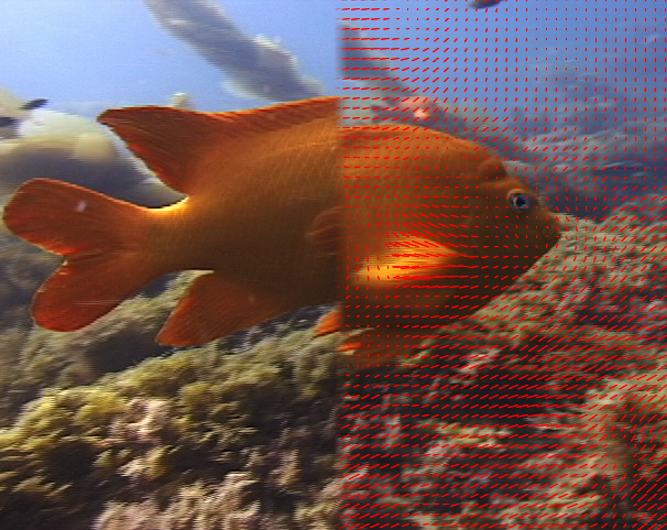
\includegraphics[width=80mm, keepaspectratio]{figures/opticalflow.png}
\caption{A kép jobb oldalán piros nyilak jelképezik az optikai áramlást.\\Forrás: \url{http://href.hu/x/dz36}}
\label{fig:optical_flow}
\end{figure}

Az eljárás feltételezi, hogy az áramlás konstans a vizsgált képpont helyi környezetében, és ebben a környezetben (ablakban) a legkisebb négyzetek módszerével próbálja kiszámolni az aktuális pont elmozdulásvektorát. Azzal, hogy nem egy-egy képpontot, hanem egy kis lokális ablakot vesz figyelembe a számítás során, a Lucas--Kanade eljárás kevésbé érzékenyen reagál a zajos képekre. Másrészt viszont a lokális tulajdonság hatására az eljárás nem tud információt szolgáltatni a kép nagy, összefüggő, azonos intenzitású területein.

%. . . . . . . . . . . . . . . . . . . . . . . . . . . . . . . . . . . . . .
\subsubsection{Matematikai háttér}\label{sect:matrixok}
%. . . . . . . . . . . . . . . . . . . . . . . . . . . . . . . . . . . . . .

Tegyük fel, hogy két egymás követő időpillanatban a képek közti eltérés megfelelően kicsi. Az optikai áramlás eljárás alapegyenlete ebben az esetben következő

\begin{align}\label{eq:optflow_alap}
I_x V_x + I_y V_y = - I_t
\end{align}

formában írható fel, ahol $V_x$ és $V_y$ az $(x,y,t)$ képpont sebességének (vagyis optikai áramlásának) $x$ és $y$ koordinátái, $I_x$, $I_y$ és $I_t$ pedig a kép parciális deriváltjai.

A Lucas--Kanade eljárásban egy, a vizsgált képpont körüli ablak tartalmát vesszük figyelembe, és feltesszük, hogy az áramlás ezen a régión belül állandó. A \eqref{optflow_alap} egyenletet ennek megfelelően a következő formára hozhatjuk

\begin{align}\label{eq:optflow_lk}
I_x(q_1)V_x + I_y(q_1)V_y &= - I_t(q_1) \nonumber \\
I_x(q_2)V_x + I_y(q_2)V_y &= - I_t(q_2) \nonumber \\
&\vdots \nonumber \\
I_x(q_n)V_x + I_y(q_n)V_y &= - I_t(q_n)
\end{align}

amelyben $q_1$, $q_2$, $\ldots$, $q_n$ az aktuálisan vizsgált pont körüli ablak egyes képpontjai.

A \eqref{optflow_lk} egyenletet $Av = b$ formában, mátrixokkal is felírhatjuk, ekkor 

\begin{align}\label{eq:optflow_matrix}
A &= \left[ \begin{array}{cc} I_x(q_1) & I_y(q_1) \\ I_x(q_2) & I_y(q_2) \\ \vdots & \vdots \\ I_x(q_n) & I_y(q_n) \end{array} \right] \nonumber \\
v &= \left[ \begin{array}{c} V_x \\ V_y \end{array} \right] \nonumber \\
b &= \left[ \begin{array}{c} -I_t(q_1) \\ -I_t(q_2) \\ \vdots \\ -I_t(q_n) \end{array} \right]
\end{align}

A \eqref{optflow_matrix}-ban definiált egyenletrendszer felülhatározott, vagyis több egyenlet szerepel benne, mint ismeretlen. A Lucas--Kanade algoritmus a legkisebb négyzetek módszerével számítja ki a sebességkomponenseket, vagyis

\begin{align}\label{eq:optflow_seb1}
v &= \frac{A^T b}{A^T A}
\end{align}

ami \eqref{optflow_matrix}-at behelyettesítve a következő alakra hozható

\begin{align}\label{eq:optflow_seb2}
\left[ \begin{array}{c} V_x \\ V_y \end{array} \right] &= \left[ \begin{array}{cc} \sum_{i=1}^n I_x(q_i)^2 & \sum_{i=1}^n I_x(q_i)I_y(q_i) \\ \sum_{i=1}^n I_x(q_i)I_y(q_i) & \sum_{i=1}^n I_y(q_i)^2 \end{array} \right]^{-1} \left[ \begin{array}{c} - \sum_{i=1}^n I_x(q_i)I_t(q_i) \\ - \sum_{i=1}^n I_y(q_i)I_t(q_i) \end{array} \right]
\end{align}

vagyis az aktuálisan vizsgált $q_1$, $q_2$, $\ldots$, $q_n$ pontokat tartalmazó ablak $p$ középpontjának $x$ és $y$ irányban vett sebességkomponenseit adja meg közvetlenül a \eqref{optflow_seb2} egyenlet.

%............................................................................
\subsection{Összegzés}\label{sect:detect_osszefoglalas}
%............................................................................

A \sectref{viola} szakaszban felsorolt eljárásoknak köszönhetően a Viola--Jones objektumdetektor képes az elődeinél jóval gyorsabban osztályozni a bemenetére küldött képeket. Ha azonban nem is lehetséges a videofolyam minden egyes képkockáján a rendelkezésre álló időn belül önállóan döntést hozni, valamilyen kiegészítő technika használatával (pl. a felismert objektumok optikai áramlás-alapú követése) \emph{valós idejű} objektumdetektáló rendszer létrehozása válik lehetővé.

A Lucas--Kanade optikai áramlás-alapú követés jó kiegészítésként szolgálhat egy nagyobb számításigényű objektumdetektor mellé. Azonban a használat során a két módszer egymáshoz viszonyított ideális összetételének megtalálása döntő a követés pontossága és gyorsasága szempontjából. 




\newpage
%,,,,,,,,,,,,,,,,,,,,,,,,,,,,,,,,,,,,,,,,,,,,,,,,,,,,,,,,,,,,,,,,,,,,,,,,,,,,
\section{Blob-műveletek}\label{sect:blob}
%,,,,,,,,,,,,,,,,,,,,,,,,,,,,,,,,,,,,,,,,,,,,,,,,,,,,,,,,,,,,,,,,,,,,,,,,,,,,

A képfeldolgozásban a \emph{blob} fogalmat a szó ,,folt'' értelmében használják, nem keverendő össze az adatbázisok BLOB (Binary Large Object -- nagy bináris objektum) fogalmával. Egy \emph{blob} informálisan a következő módon definiálható:

\begin{definition}
A képtér valamely tulajdonság egyezősége, vagy korlátozott mértékű eltérése alapján összetartozó régióját \textbf{blob}-nak nevezzük.
\end{definition}

A definícióban említett tulajdonság a gyakorlatban legtöbbször a képpontok színe vagy intenzitása. Azonban más, nem RGB színtérben reprenzentált képek esetén egyéb tulajdonság szerinti összetartozás is hasznos információt hordozhat (pl. a HSV színtérben vett szaturáció).

\bigskip

A szakirodalomban két eljárást tartanak számon a blob-ok meghatározásával kapcsolatban. A \textbf{blob-detektálás} (blob detection) differenciális vagy lokális szélsőértékeken alapuló metódusok segítségével keresi a képtér érdekes pontjait, legszélesebb körben a \emph{Laplacian of the Gaussian (LoG)} operátort használva. A blob-detektálás olyan további információkat szolgáltathat az él- és sarokdetektáló algoritmusok mellé, amelyek elősegíthetik a kép feldolgozását illetve megértését, teret pontosabb nyitva objektumfelismerési és -követési módszerek fejlesztésének.

A blob-detektálással rokon, de attól független eljárás a \textbf{komponens-címkézés}. A módszer több néven is ismert, pl. régió-címkézés, blob-címkézés, komponens-analízis. A gépi látás terén komponens-címkézésen legtöbbször két dimenziós bináris képek összetartozó régióinak -- ezek a blob-ok -- felkutatását és elkülönítését értjük, de a későbbiekben bemutatott elvek kiterjeszthetők szürkeárnyalatos vagy színes képek, illetve akár többdimenziós adathalmazok elemzésére is.

\bigskip

Munkám során a bináris képek feldolgozása került előtérbe, ennek megfelelően a továbbiakban a címkézéssel kapcsolatos elméleti alapokat foglalom össze. A \sectref{blob_cimke}~szakaszban a címkézési algoritmusokat ismertetem, majd a \sectref{blob_analizis}~szakaszban áttekintem azokat a jellemzőket, amelyek hasznosnak bizonyulhatnak a blob-ok osztályozása és szűrése során.

%............................................................................
\subsection{Komponens-címkézés}\label{sect:blob_cimke}
%............................................................................

Az egyszerűség kedvéért a komponens-címkézés alapelvét két dimenziós képek esetén mutatom be. Könnyen belátható, hogy a későbbiekben ismeretett módszerek egyszerűen kiterjeszthetők többdimenziós halmazok címkézésére is -- természetesen az idő- és tárigény növekedése mellett.

\bigskip

A címkézés megkezdése előtt minden esetében fontos, hogy megszabjuk a használni kívánt \textbf{szomszédosság-mértéket}. Ez a címkézés során a legtöbbször 4- vagy 8-szomszédosságot jelent. A \textbf{4-szomszédossági} esetben egy pixel szomszédait a tőle $N$, $W$, $S$ és $E$ irányban lévő képpontok jelentik az égtájak angol elnevezései alapján. \textbf{8-szomszédosság} használatakor a képponthoz csak a sarkával illeszkedő pontokat is szomszédnak vesszük, tehát az óramutató járásával ellentétes irányban $N$, $NW$, $W$, $SW$, $S$, $SE$, $E$ és $NE$ szomszédokról beszélhetünk.

\bigskip

A feladat tehát olyan algoritmust találni, amely lehetőleg minél kisebb számítási komplexitással képes adott szomszédosság-mérték mellett elkülöníteni képeken az összetartozó régiókat.

%. . . . . . . . . . . . . . . . . . . . . . . . . . . . . . . . . . . . . .
\subsubsection{Kétlépéses algoritmusok}\label{sect:blob_ketlepes}
%. . . . . . . . . . . . . . . . . . . . . . . . . . . . . . . . . . . . . .

A kétlépéses (two-pass) algoritmusok -- nevükből adódóan -- két különálló lépésben határozzák meg a bináris képen található összefüggő blob-okat.

\begin{enumerate}
  \item Első lépésben \textbf{átmeneti címkék} kiosztására, valamint az átmeneti címkék közti ekvivalenciák meghatározására kerül sor.
  \item Második lépésben már meghatározhatjuk a komponenseket a korábban ekvivalensnek jelzett címkék \textbf{összevonásával}.
\end{enumerate}


%.  .  .  .  .   .  .  .  .  .  .  .  .  .  .  .  .  .  .  .  .  .  .  .  .  . . . . . . . . . . . . 
\paragraph{Rosenfeld--Pfalz}
%.  .  .  .  .   .  .  .  .  .  .  .  .  .  .  .  .  .  .  .  .  .  .  .  .  . . . . . . . . . . . . 

A klasszikus algoritmus \cite{rosenfeld} mindkét lépésben sorra veszi a képtér pontjait balról-jobbra, majd fentről lefelé haladva. Ebben a konfigurációban az összetartozóságot az aktuálisan vizsgált képpontra

\begin{itemize}
  \item 4-szomszédosság esetén az $N$ és $W$ szomszéd,
  \item 8-szomszédosság esetén az $NE$, $N$, $NW$ és $W$ szomszédok
\end{itemize}

vizsgálatával döntjük el. Az algoritmust 4-szomszédosságot feltételezve ismertetem.

\bigskip

Az \textbf{első lépés} során az algoritmus minden képppont esetén a következő négy feltétel vizsgálatát végzi el, és az eredménynek megfelelően látja el a pontot átmeneti címkével. Egy feltétel teljesülése esetén a vizsgálat leáll, egyébként a következő feltétel vizsgálata következik.

Bár egyértelműnek tűnik, de érdemes megjegyezni, hogy az algoritmus leírásában megkülönböztetjük a képpontok \emph{értékét} (bináris képek esetén a hátteret figyelmen kívül hagyva ez egyetlen értéket jelent), valamint a hozzájuk rendelt \emph{címkét}!

\bigskip

Az éppen vizsgálat alatt lévő pontot jelölje $P$, a képpont értékét megadó függvényt $v$, a címkézést definiáló függvényt pedig $c$. A régiók címkéit jelöljük növekvő pozitív egész számokkal.

\begin{enumerate}
% ---
% elso
  \item feltétel: $v(P) = v(W)$ \\ \begin{small} $W$ szomszéd értéke megegyezik a vizsgált pont értékével. \end{small}   
    \begin{itemize}
      \item $c(P) := c(W)$ \\ \begin{small} Mindenképpen azonos régióban vagyunk, alkalmazzuk $P$-re $W$ címkéjét! \end{small}
    \end{itemize}
 
% ---
% masodik
  \item feltétel: $v(W) = v(N)$ és $c(W) \neq c(N)$ \\ \begin{small}$W$ és $N$ szomszéd értéke megegyezik, de címkéjük különböző. \end{small}
    \begin{itemize}
      \item $c(P) := min \lbrace c(W), c(N)\rbrace$ \\ \begin{small}A két szomszédnak nyilvánvalóan egy régióba kellene tartoznia. Alkalmazzuk a kisebbik címkét, és \textbf{jegyezzük fel a címkék ekvivalenciáját}!\end{small}
    \end{itemize}

% ---
% harmadik
  \item feltétel: $v(W) \neq v(P)$ és $v(N) = v(P)$ \\ \begin{small}$W$ értéke különbözik, de $N$ értéke megegyezik vizsgált pont értékével. \end{small}
    \begin{itemize}
      \item $c(P) := c(N)$ \\ \begin{small}Alkalmazzuk az $N$ szomszéd címkéjét!\end{small}
    \end{itemize}

% ---
% negyedik
  \item feltétel: $v(W) \neq v(P)$ és $v(N) \neq v(P)$  \\ \begin{small}$W$ és $N$ értéke különbözik $P$ értékétől.\end{small}
    \begin{itemize}
      \item $c(P) := max \lbrace c \rbrace + 1$ \\ \begin{small}Készítsünk egy új címkét és alkalmazzuk!\end{small}
    \end{itemize}

\end{enumerate}

A \textbf{második lépésben} az algoritmus újra végigiterál a képpontokon, és minden képpont címkéjét az ekvivalensnek jelzett címkék közül a legkisebbel helyettesíti.

A megvalósítás során az algoritmus \emph{diszjunk-halmaz erdő} (disjoint-set) adatszerkezetet használ, amely ideális a régiók közti ekvivalenciák tárolására és elérésére. 


%.  .  .  .  .   .  .  .  .  .  .  .  .  .  .  .  .  .  .  .  .  .  .  .  .  . . . . . . . . . . . . 
\paragraph{Lifeng-Yuyan-Suzuki}
%.  .  .  .  .   .  .  .  .  .  .  .  .  .  .  .  .  .  .  .  .  .  .  .  .  . . . . . . . . . . . . 

A szerzők által 2008-ban prezentált algoritmus \cite{suzuki} a klasszikusnál gyorsabb feldolgozást tesz lehetővé. Az előzőekhez hasonlóan itt is két lépésben iterálunk végig a képen balról-jobbra, fentről-lefelé, a háttérhez tartozó képpontokat figyelmen kívül hagyva.

\bigskip

Az \textbf{első lépés} során elvégzendő feladatok az aktuális képpontra:

\begin{enumerate}
  \item Vizsgáljuk a képpont szomszédait, a szomszédosság-mértéknek megfelelően!
  \item Ha nincsenek szomszédok (mind a háttérhez tartozik), rendeljünk új címkét az elemhez és folytassuk az algoritmust a következő képponttal!
  \item Ha vannak szomszédok, címkézzük a képpontot a legkisebb szomszédos címkével!
  \item Tároljuk a szomszédos címkék közti ekvivalenciákat!
\end{enumerate}

A \textbf{második lépésben}, hasonlóan az előző megoldáshoz, a képpontokat újra sorba véve újracímkézzük azokat az ekvivalens címkék legkisebbikével.

%. . . . . . . . . . . . . . . . . . . . . . . . . . . . . . . . . . . . . .
\subsubsection{Egyéb algoritmusok}\label{sect:blob_egyeb}
%. . . . . . . . . . . . . . . . . . . . . . . . . . . . . . . . . . . . . .

A komponens-címkézés problémájára a \sectref{blob_ketlepes}~szakaszban taglaltakon kívül is számos más megoldás született. Léteznek a feldolgozást összevonó egylépéses (one-pass) algoritmusok, de olyan többlépéses (multi-pass) algoritmust is kifejlesztettek már, amely lineáris komplexitással oldja meg a feladatot. \cite{suzuki_lin}

Az egyesével, szinte egymástól függetlenül vizsgált képpontok feldolgozása párhuzamosításért kiált: párhuzamosított komponens-címkéző algoritmusok fejlesztésére is sor került \cite{comp_parallel}, és a téma továbbra is nagy érdeklődésre tart számot a párhuzamosított számítási platformok (pl. CUDA, OpenMP) előretörésével.

%............................................................................
\subsection{Blob-analizis}\label{sect:blob_analizis}
%............................................................................

Sok esetben a képen felismert blob-ok nem mindegyik tartalmaz a feldolgozás szempontjából hasznos információt. A blob-ok algoritmikus megtalálása mellett szükségünk lehet a foltok által hordozott absztrakt információ megértésére is. A feladat elvégzéséhez hasznunkra válhat olyan mértékek meghatározása, amelyekkel \textbf{szűrni tudjuk} a felismert blob-okat valamely előre definiált kritérium alapján.

A pupillakeresési feladatnál például az ember számára könnyen feldolgozható \emph{,,keressünk egy relatíve nagy, kör alakú objektumot''} feltételt kell a gépi látás által is megoldható problémává formalizálni.

Nem feltétlenül kell azonban rögtön komplex mértékek felhasználásába bonyolódnunk. Jól megfogalmazott kritérium esetén sokszor a legegyszerűbb jellemzők is segítségünkre lehetnek: legyen szó akár egyszerű zajszűrésről, vagy a feldolgozás szempontjából fontos blob-ok azonosításáról.

\bigskip

Az egyszerűbb mértékek közé tartoznak az objektum kiterjedésével és kerületével kapcsolatos jellemzők.

\begin{itemize}
  \item \textbf{terület}
    \begin{itemize}
      \item objektum területe
      \item lyukak száma és területe
      \item teljes terület \\ \begin{small}(objektum plusz lyukak területe)\end{small}
    \end{itemize}
  \item \textbf{kerület}, vagyis a kontúr hossza
  \item \textbf{befoglalók}
    \begin{itemize}
      \item befoglaló keret (bounding box) \\ \begin{small}(pl. két ellentétes sarok megadásával)\end{small}
      \item elforgatott befoglaló keret \\ \begin{small}(pl. középpont, szélesség/magasság valamint irányszög megadásával)\end{small}
      \item konvex héj (convex hull) \\ \begin{small}(pontjai megadásával)\end{small}
      \item befoglaló ellipszis \\ \begin{small}(pl. középpont, kis-, nagytengely, irányszög megadásával)\end{small}
    \end{itemize}
\end{itemize}

\bigskip

A blob-ok képen belüli elhelyezkedésének meghatározásakor lehet hasznos a blob \textbf{súlypontjának} meghatározása.

\begin{definition}{Súlypont:}
$x_m = \dfrac{\sum_{i=1 \dots N} x_i}{N}$ és $y_m = \dfrac{\sum_{i=1 \dots N} y_i}{N}$, ahol $N$ a blob-hoz tartozó képpontok száma
\end{definition}

\bigskip

A szabályos formáktól való eltérés mértékét határozhatjuk meg a \textbf{kompaktság} definiálásával. Jelölje $P$ a kerületet, $A$ a területet, valamint $W$ és $H$ a befoglaló téglalap szélességét és magasságát.

\begin{definition}{Kompaktság 1:}
$\dfrac{P^2}{A}$ $\Longrightarrow$ diszkre minimális
\end{definition}

\begin{definition}{Kompaktság 2:}
$\dfrac{A}{W \cdot H}$ $\Longrightarrow$ téglalapra minimális
\end{definition}

\bigskip

A befoglaló keret (bounding box) szélesség/hosszúság aránya az objektum általánosságban vett \textbf{elnyújtottságáról} ad információt. 

\begin{definition}{Elnyújtottság:}
$\dfrac{W}{H}$
\end{definition}

\bigskip

Az objektum \textbf{körkörösségét} (Heywood Circularity Factor) is könnyen definiálhatjuk a kerület és a terület felhasználásával. A képlet tökéletesen kör alakú objektumra $1$ értéket ad vissza.

\begin{definition}{Körkörösség:}
$\dfrac{P}{2 \sqrt{\pi A}}$
\end{definition}

\bigskip

A blob orientációjának meghatározásában lehet segítségünkre a \textbf{Feret-átmérő} fogalma. Az általános definíció szerint Feret-átmérőn azt a értéket értjük, amely távolságba az objektum ,,beszorítható'' a megadott iránnyal párhuzamos egyenesek közé. A fogalom legkönnyebben úgy szemlélethető, mintha az objektumot egy tolómérő adott irányba álló pofái közé szorítanánk. A tolómérőn leolvasott érték az objektum mérési irányra vett Feret-átmérője -- ebből származik a másik, főlet angolszász területen elterjedt elnevezés, a \emph{caliper diameter} (caliper: tolómérő, tolómérce). 

A gépi látás területén Feret-átmérőn általában automatikusan a legnagyobb Feret-átmérőt értjük. A legnagyobb Feret-átmérő irányszögét kitűnően használhatjuk a blob \textbf{orientációjának} jellemzésére.

%............................................................................
\subsection{Összegzés}\label{sect:blob_osszegzes}
%............................................................................

asdf